\section{Optimization Benchmark Analysis}

Optimization behavior cannot be judged from a single learning curve or from an optimizer name in isolation. A meaningful comparison must control the model, objective, preprocessing, regularization, data split, stopping rule, and numerical precision, because any of these factors can dominate the apparent difference between optimizers. The purpose of this case study is therefore not to crown a universal optimizer, but to show how optimizer choice changes when the geometry of the objective, the conditioning of the feature representation, and the computational regime change.

The study begins with a controlled convex benchmark because convex logistic regression separates optimization behavior from model nonconvexity. The Wisconsin Diagnostic Breast Cancer dataset provides a compact public classification problem on which first-order and quasi-Newton methods can be compared under the same regularized logistic objective. This controlled setting makes it possible to measure convergence speed, held-out discrimination, calibration-related loss, and sensitivity to feature conditioning without attributing differences to architecture changes or stochastic data pipelines.

The controlled experiment is then used as an anchor for the broader regimes developed in the surrounding worked examples: convolutional networks, transformer pretraining, physics-informed neural networks, and reinforcement learning. Those regimes introduce nonconvexity, optimizer-state memory, distributed communication, composite residual losses, and nonstationary data collection. The central lesson is that optimizer selection is an engineering decision conditioned on objective geometry and system constraints rather than a fixed ranking that transfers unchanged across tasks.

\subsection{Case Study: Cross-Domain Optimizer Selection}

Optimizer selection is often discussed as though an optimizer has a task-independent ranking, but this is not supported by either optimization theory or engineering practice. Curvature, stochasticity, numerical conditioning, regularization, batch construction, and system constraints all interact with the update rule. A defensible case study must therefore separate optimization efficiency from predictive generalization and must expose the numerical assumptions under which a method succeeds.

The controlled benchmark in this section uses convex logistic regression because it provides a setting in which all methods optimize the same objective and architectural confounders are absent. That controlled setting is especially useful for identifying when rapid objective reduction does not translate into stronger held-out performance, and for observing how deliberately degraded feature conditioning changes optimizer behavior.

The broader interpretation then connects the controlled findings to the chapter's nonconvex worked examples. Convolutional networks, transformers, physics-informed neural networks, and reinforcement-learning policies introduce different objective geometries and systems constraints, so the convex benchmark is used as a diagnostic anchor rather than as evidence for a universal optimizer ranking.

\textbf{Objective:} The objective is to determine how optimizer behavior changes when model, objective, preprocessing, regularization, data splits, and stopping criteria are held fixed, and to separate fast objective reduction from held-out predictive performance and numerical robustness.

\textbf{Problem:} The scientific question is how first-order, adaptive, momentum-based, and quasi-Newton optimization differ when the predictive model and loss are held fixed, and how those conclusions change as numerical conditioning deteriorates. The controlled benchmark isolates optimizer behavior on a convex objective before the discussion extends the interpretation to nonconvex and distributed regimes.

\textbf{Dataset:} The quantitative benchmark uses the Wisconsin Diagnostic Breast Cancer dataset distributed with scikit-learn, containing 569 observations and 30 real-valued features. Each run uses a stratified 75/25 train-test split. Three fixed random seeds are used (7, 19, 41). Features are standardized using statistics computed only from the training partition. The conditioning experiment uses the same dataset but applies controlled feature rescaling after root-mean-square normalization to produce increasingly ill-conditioned design matrices without changing labels or sample membership.

\textbf{Model:} All quantitative comparisons use the same regularized binary logistic-regression model. SGD, momentum, and AdamW-style first-order updates are implemented directly in NumPy, while L-BFGS is implemented with SciPy's L-BFGS-B solver. This shared objective prevents architectural differences from being confused with optimizer effects.

\textbf{Method:} The primary benchmark records training binary cross-entropy over optimization steps and evaluates balanced accuracy, ROC--AUC, held-out log loss, elapsed optimization time, and the number of optimization steps. Results are aggregated over the three fixed stratified splits. The conditioning study multiplies a fixed block of normalized features by factors of 1, 3, 10, 30, and 100, measures the condition number of the regularized feature Gram matrix, and records whether SGD or L-BFGS reaches the same training-loss threshold within a 400-step budget.

\textbf{Metrics:} The primary metrics are training binary cross-entropy, optimization steps to a fixed loss threshold, held-out balanced accuracy, ROC--AUC, test log loss, and conditioning sensitivity.  Figure~\ref{fig:ch1-optimizer-selection-benchmark} separates optimization behavior from predictive behavior. Panel (a) reports the mean training-loss trajectory with one-standard-deviation bands across the three splits; panel (b) reports mean held-out balanced accuracy with one-standard-deviation error bars. Figure~\ref{fig:ch1-optimizer-conditioning} then tests sensitivity to numerical conditioning: panel (a) reports the optimization steps required to reach the fixed training-loss threshold, capped at 400 steps, and panel (b) reports held-out balanced accuracy over the same conditioning sweep. Tables~\ref{tab:ch1-optimizer-benchmark} and~\ref{tab:ch1-conditioning-benchmark} provide the corresponding numerical summaries.

\begin{figure}[t]
\centering
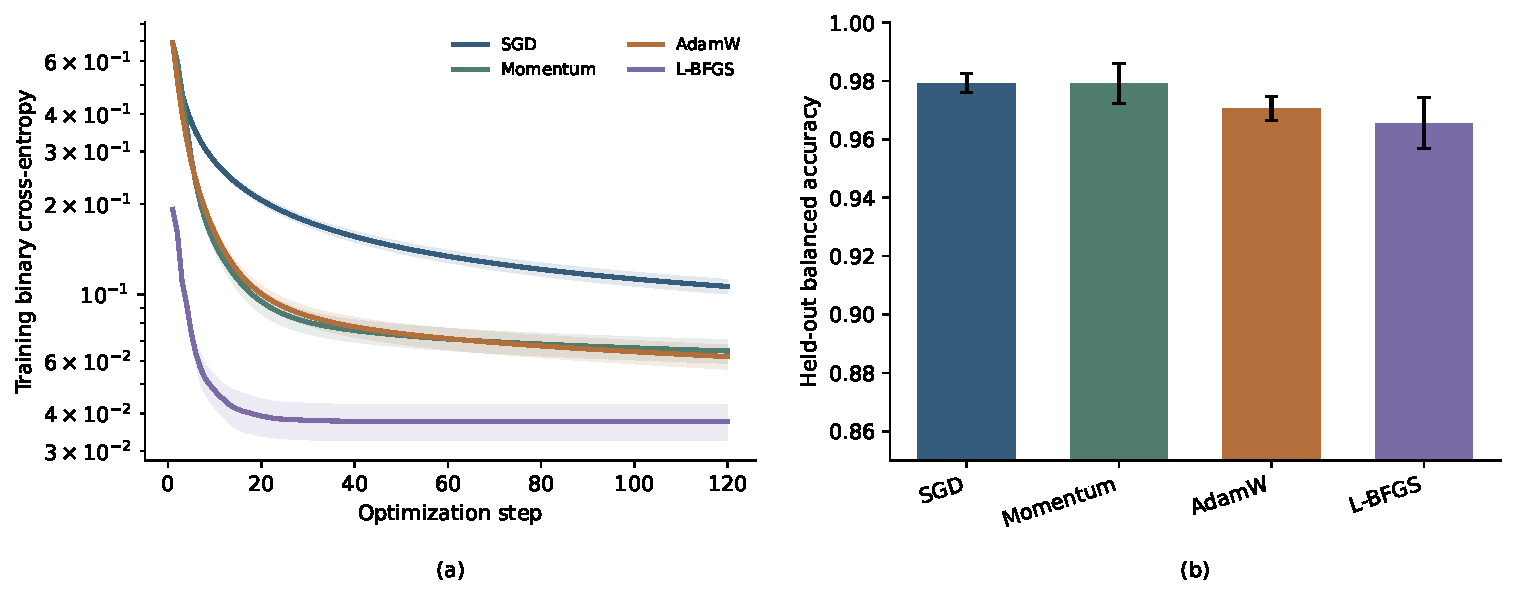
\includegraphics[width=\BookFigureWidth]{figures/ch01_optimizer_selection_benchmark.pdf}
\caption{Controlled optimizer benchmark on the Wisconsin Diagnostic Breast Cancer dataset using the same regularized logistic-regression objective for every method. (a) Mean training binary cross-entropy across three stratified train-test splits; shaded bands show one standard deviation. L-BFGS reduces the training objective rapidly, whereas the first-order methods descend more gradually over the fixed step budget. (b) Held-out balanced accuracy for the same runs, reported as mean $\pm$ one standard deviation. Rapid objective reduction does not automatically imply the best held-out classification performance, illustrating why optimizer comparisons must report both optimization and generalization metrics.}
\label{fig:ch1-optimizer-selection-benchmark}
\end{figure}

\begin{table}[t]
\centering
\small
\caption{Controlled optimizer comparison on the Wisconsin Diagnostic Breast Cancer dataset. Values are means over three fixed stratified splits; uncertainty for balanced accuracy is one standard deviation. All methods optimize the same regularized logistic objective.}
\label{tab:ch1-optimizer-benchmark}
\begin{tabular}{lrrrrr}
\toprule
Optimizer & Steps & Train loss & Balanced accuracy & ROC--AUC & Test log loss \\
\midrule
SGD      & 250.0 & 0.0863 & $0.9793 \pm 0.0032$ & 0.9959 & 0.0792 \\
Momentum & 250.0 & 0.0584 & $0.9793 \pm 0.0068$ & 0.9960 & 0.0609 \\
AdamW    & 250.0 & 0.0530 & $0.9706 \pm 0.0040$ & 0.9946 & 0.0760 \\
L-BFGS   & 119.7 & 0.0377 & $0.9656 \pm 0.0086$ & 0.9894 & 0.1567 \\
\bottomrule
\end{tabular}
\end{table}

\begin{figure}[t]
\centering
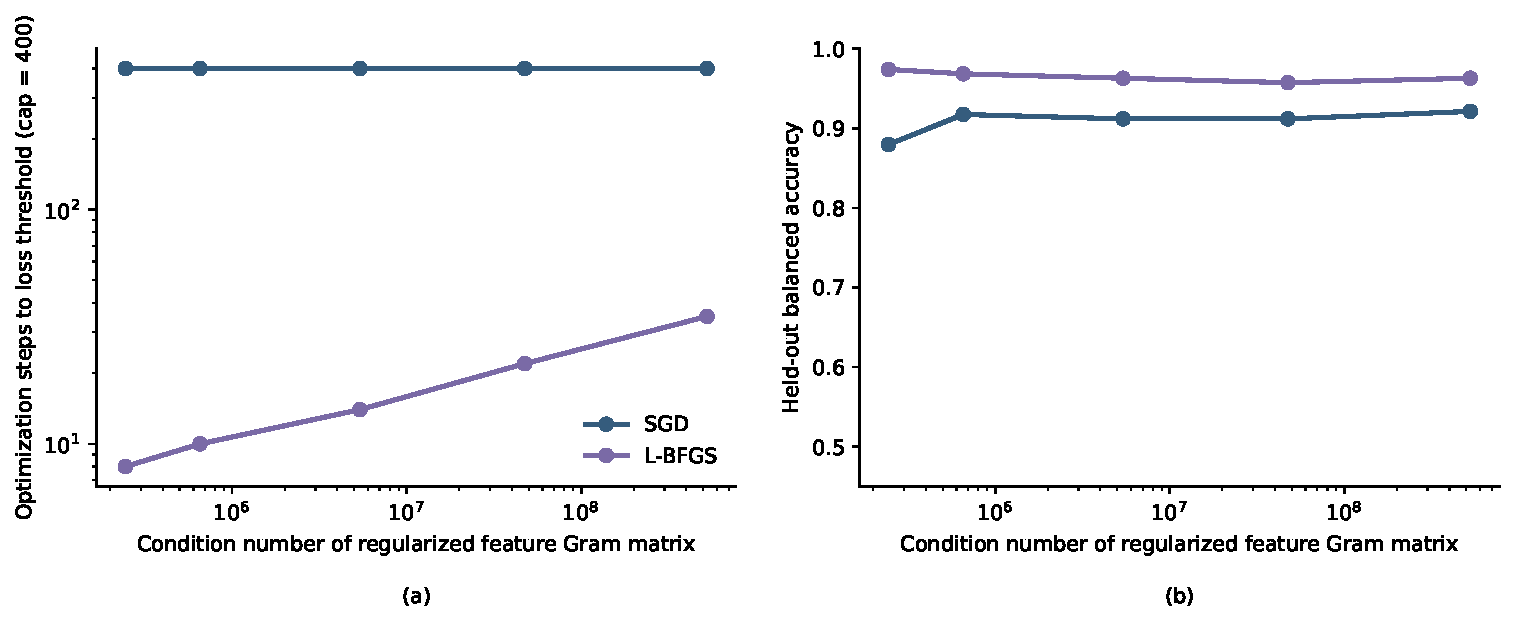
\includegraphics[width=\BookFigureWidth]{figures/ch01_optimizer_conditioning_sensitivity.pdf}
\caption{Sensitivity of convex logistic-regression optimization to controlled feature conditioning on the same Wisconsin Diagnostic Breast Cancer data. (a) Optimization steps required to reach a fixed training-loss threshold as the condition number of the regularized feature Gram matrix increases; runs that do not reach the threshold are shown at the 400-step cap. (b) Held-out balanced accuracy for the corresponding models. The experiment shows that quasi-Newton acceleration is highly effective in the better-conditioned regimes but can become numerically fragile under severe feature scaling, while the conservative first-order trajectory changes more gradually.}
\label{fig:ch1-optimizer-conditioning}
\end{figure}

\begin{table}[t]
\centering
\small
\caption{Conditioning-sensitivity benchmark for SGD and L-BFGS on the controlled logistic-regression experiment. A value of 400 steps denotes the experiment cap and does not imply that the loss threshold was reached.}
\label{tab:ch1-conditioning-benchmark}
\begin{tabular}{rrrrrr}
\toprule
Scale factor & Condition number & Optimizer & Steps & Final train loss & Balanced accuracy \\
\midrule
1   & $2.44\times10^{5}$ & SGD    & 400 & 0.4556 & 0.8796 \\
1   & $2.44\times10^{5}$ & L-BFGS & 9   & 0.1154 & 0.9384 \\
3   & $6.55\times10^{5}$ & SGD    & 400 & 0.2843 & 0.9173 \\
3   & $6.55\times10^{5}$ & L-BFGS & 8   & 0.1192 & 0.9267 \\
10  & $5.40\times10^{6}$ & SGD    & 400 & 0.2244 & 0.9117 \\
10  & $5.40\times10^{6}$ & L-BFGS & 14  & 0.1192 & 0.9417 \\
30  & $4.75\times10^{7}$ & SGD    & 400 & 0.1923 & 0.9117 \\
30  & $4.75\times10^{7}$ & L-BFGS & 400 & 0.6931 & 0.5000 \\
100 & $5.26\times10^{8}$ & SGD    & 400 & 0.1716 & 0.9212 \\
100 & $5.26\times10^{8}$ & L-BFGS & 400 & 0.6931 & 0.5000 \\
\bottomrule
\end{tabular}
\end{table}

\textbf{Results:} The controlled benchmark demonstrates that optimizer conclusions depend on the metric being optimized. L-BFGS reaches a substantially lower training objective in fewer optimization steps, but the first-order SGD and momentum runs achieve the strongest mean held-out balanced accuracy under this protocol. The conditioning sweep further shows that the quasi-Newton advantage is not unconditional: when feature scaling drives the Gram-matrix condition number into the most severe regime, the configured L-BFGS run fails to reach the target loss within the step budget and collapses to chance-level balanced accuracy. These measurements support a narrower and more defensible conclusion than a universal optimizer recommendation: L-BFGS can be highly efficient for suitable convex problems, but preprocessing, conditioning, and validation behavior remain part of optimizer selection.

\textbf{Error Analysis:} The largest discrepancy between training objective and held-out performance occurs for L-BFGS, which continues to reduce the regularized training loss while producing weaker test log loss than the first-order alternatives. This is a useful reminder that aggressive convergence on a small dataset can expose sensitivity to regularization and split composition. Under extreme feature rescaling, numerical conditioning becomes the dominant failure mode; the problem is no longer the absence of curvature information but the reliability of the local curvature model itself.

\textbf{Limitations:} This benchmark is deliberately small and controlled. It does not establish a universal optimizer ranking for convolutional networks, transformers, PINNs, or reinforcement learning, where stochastic minibatches, nonconvex objectives, optimizer-state memory, communication overhead, and nonstationary data collection materially change the problem. The experiment also uses a fixed regularization strength and fixed learning rates rather than an exhaustive per-optimizer hyperparameter search, so the reported values should be interpreted as a reproducible diagnostic rather than a leaderboard.

\textbf{Research Implications:} Optimizer studies should report objective convergence and held-out behavior together, disclose preprocessing and conditioning, and separate algorithmic effects from hyperparameter tuning and systems effects. The regime-specific worked examples that follow this case study use the controlled result as a reference point when discussing CNN, transformer, PINN, and reinforcement-learning optimization.
